\begin{apendicesenv}

\partapendices

\chapter{EAP} \label{apendice:eap}

\begin{figure}[h!]
	\centering
  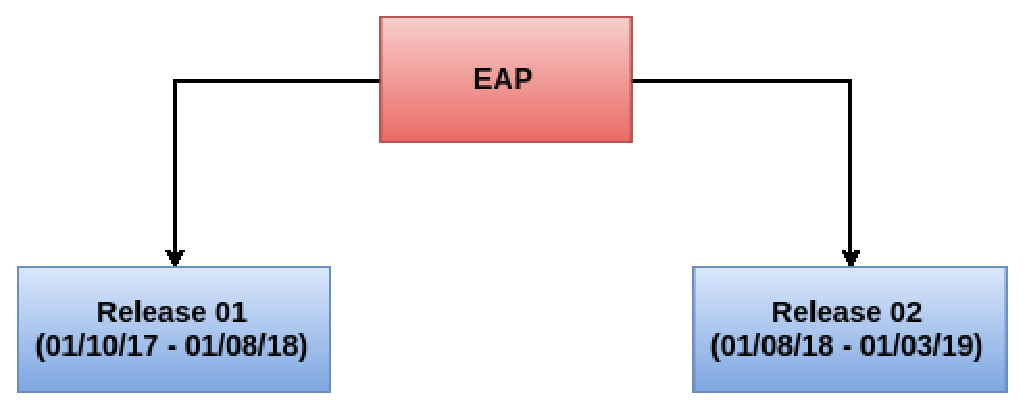
\includegraphics[keepaspectratio=true,scale=0.8]{figuras/eap1.eps}
  \caption[EAP do projeto.]{EAP do projeto. Fonte: Autor}
	\label{fig:eap}
\end{figure}

\begin{figure}[h!]
	\centering
  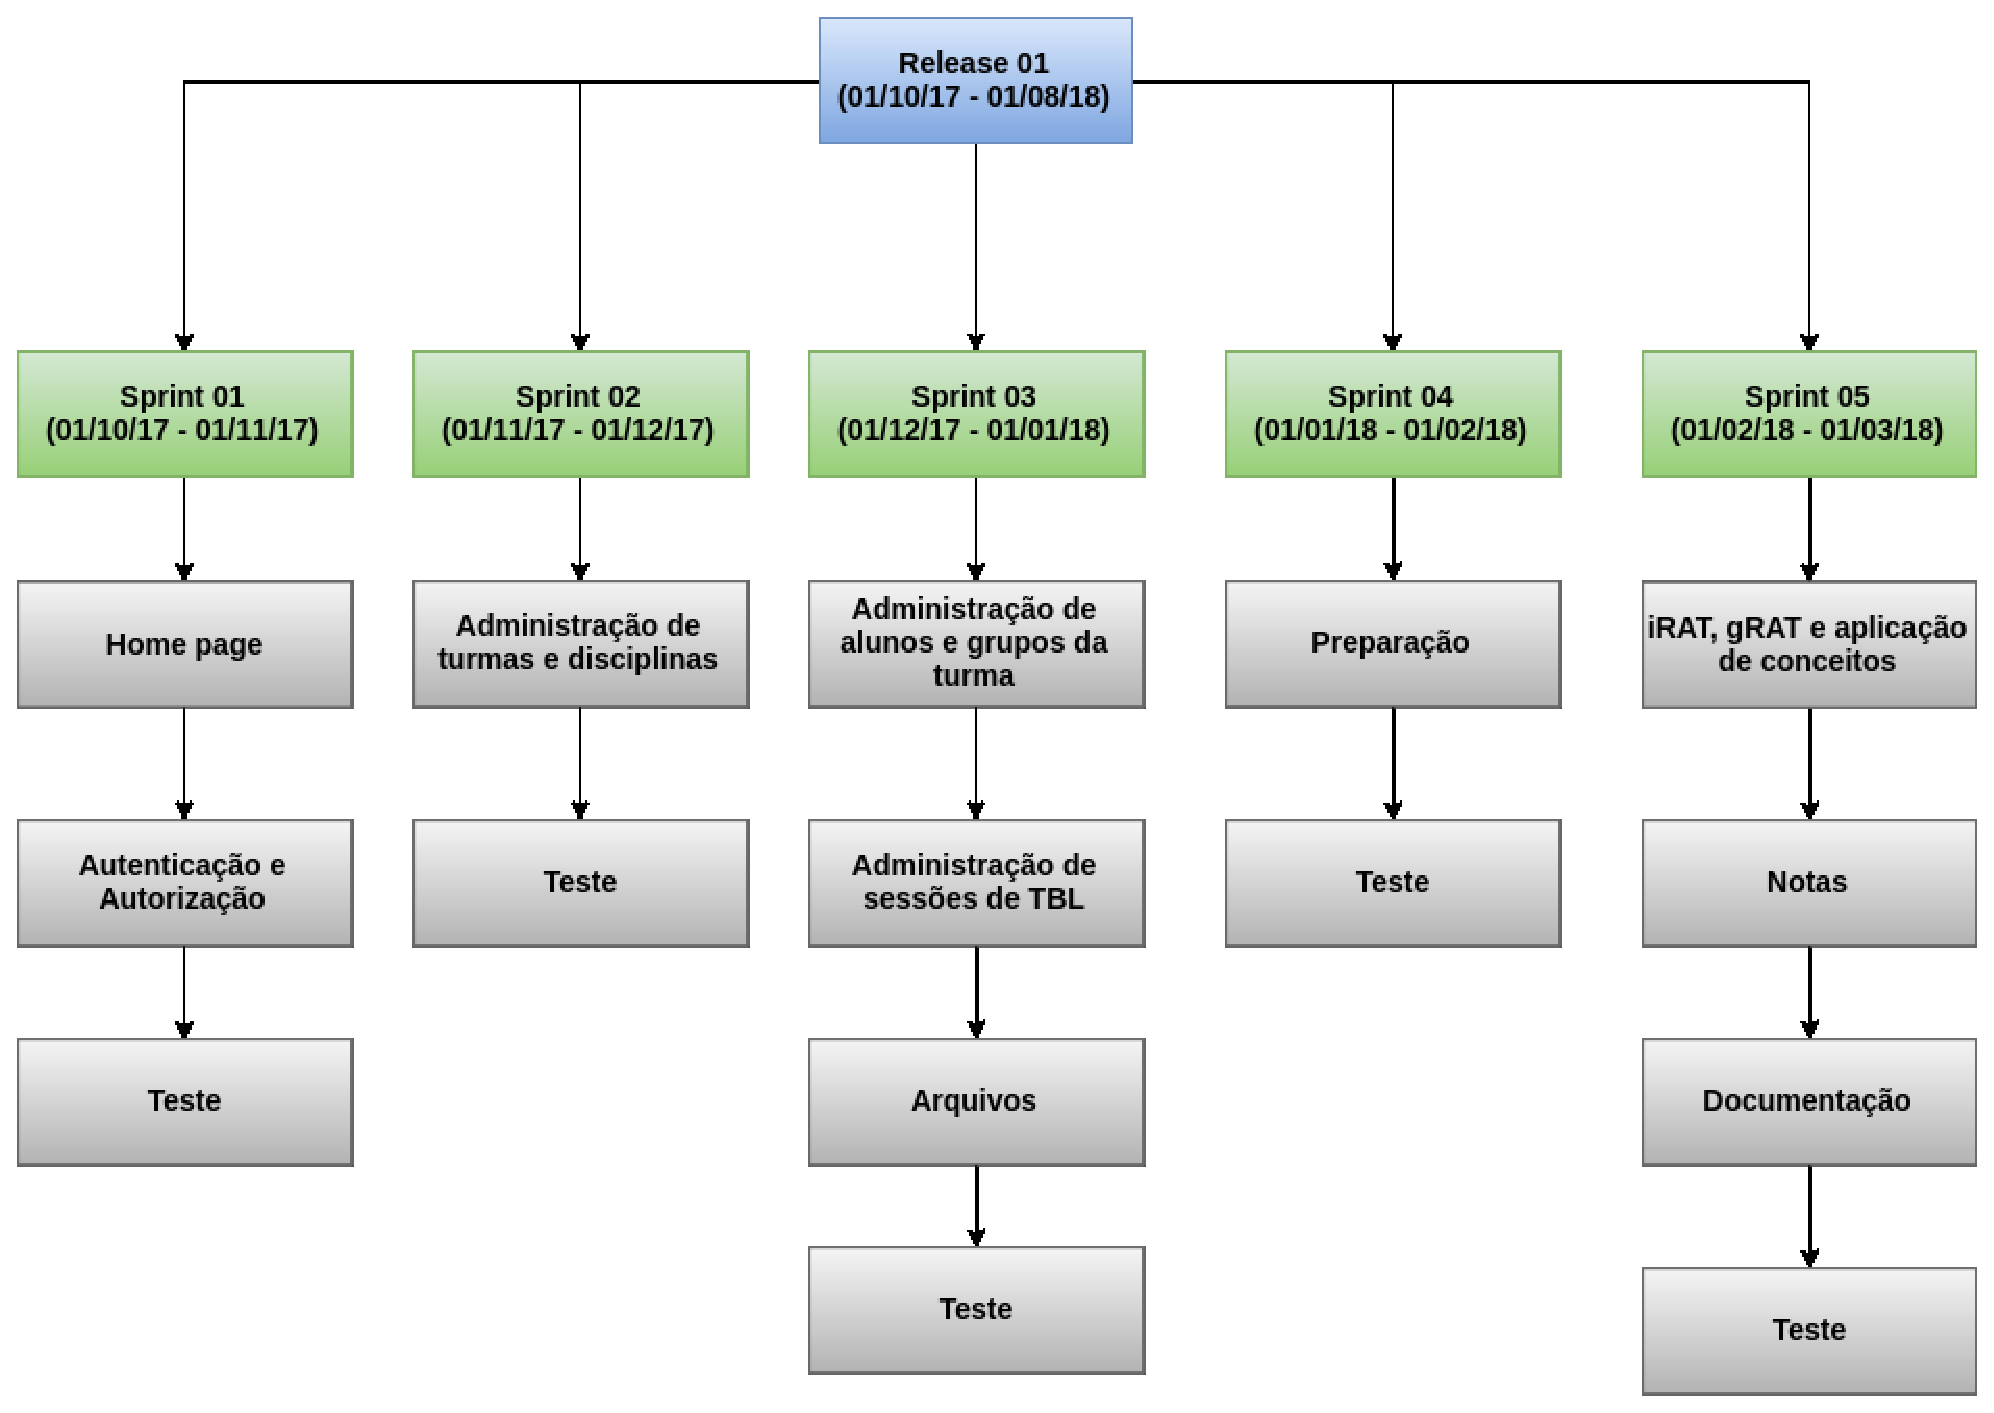
\includegraphics[keepaspectratio=true,scale=0.4]{figuras/eap2.eps}
  \caption[EAP do projeto, release 01]{EAP do projeto, release 01. Fonte: Autor}
	\label{fig:eap}
\end{figure}

\begin{figure}[h!]
	\centering
  \includegraphics[keepaspectratio=true,scale=0.4]{figuras/eap3.eps}
  \caption[EAP do projeto, release 02.]{EAP do projeto, release 02 Fonte: Autor}
	\label{fig:eap}
\end{figure}

\chapter{ROADMAP} \label{apendice:roadmap}

\begin{figure}[h!]
	\centering
  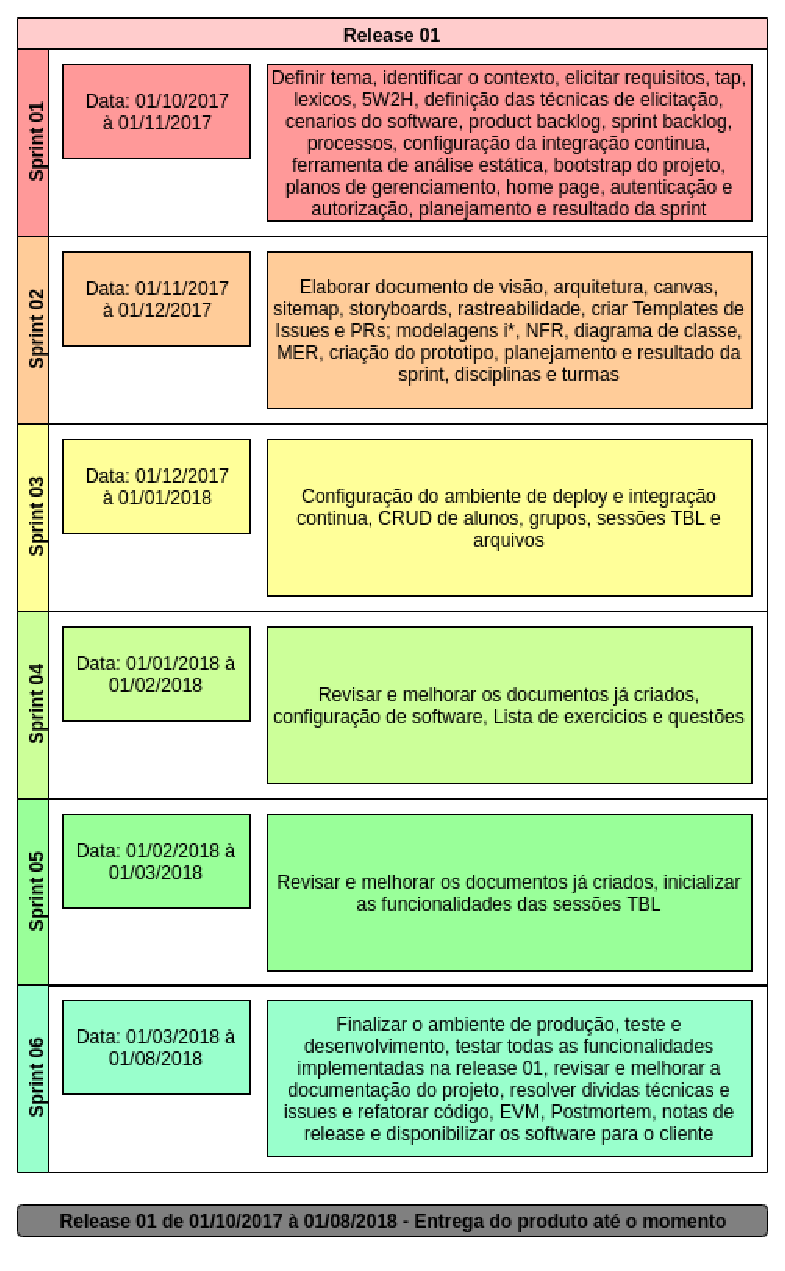
\includegraphics[keepaspectratio=true,scale=0.8]{figuras/roadmap1.eps}
  \caption[Roadmap da release 01.]{Roadmap da release 01. Fonte: Autor}
	\label{fig:roadmap1}
\end{figure}

\begin{figure}[h!]
	\centering
  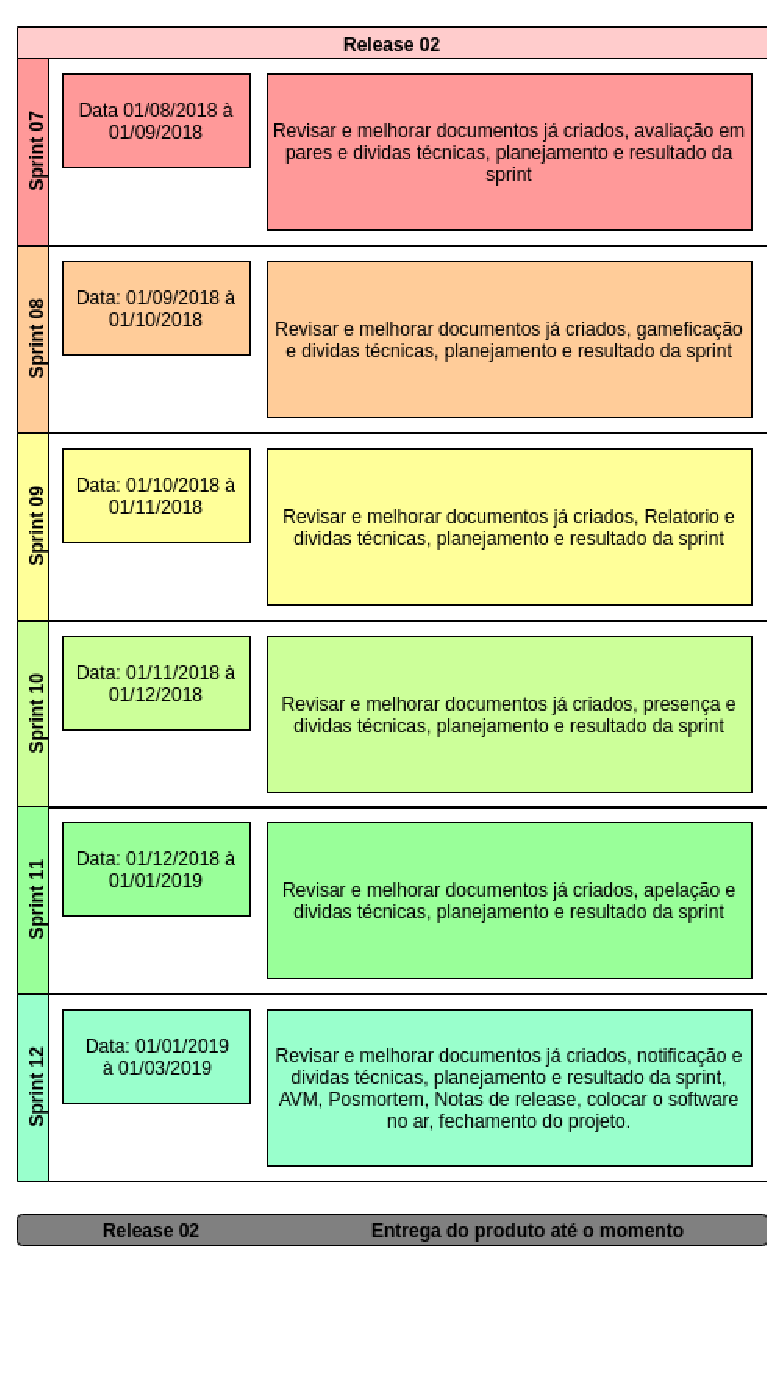
\includegraphics[keepaspectratio=true,scale=0.8]{figuras/roadmap2.eps}
  \caption[Roadmap da release 02]{Roadmap da release 02. Fonte: Autor}
	\label{fig:roadmap2}
\end{figure}

\end{apendicesenv}
